
%(BEGIN_QUESTION)
% Copyright 2006, Tony R. Kuphaldt, released under the Creative Commons Attribution License (v 1.0)
% This means you may do almost anything with this work of mine, so long as you give me proper credit

Explain what this electric solenoid valve will cause the pneumatically-actuated control valve to do when de-energized.  What sort of fail-safe mode does this solenoid provide for the control valve that the valve would not otherwise exhibit on its own?

$$\includegraphics[width=15.5cm]{i00917x01.eps}$$

Also, based on how you know liquid flow controllers are typically tuned, how will the controller (FIC) react in automatic mode if the solenoid ``trips''?

\vskip 20pt \vbox{\hrule \hbox{\strut \vrule{} {\bf Suggestions for Socratic discussion} \vrule} \hrule}

\begin{itemize}
\item{} What type of process is liquid flow: {\it self-regulating}, {\it integrating}, or {\it runaway}?
\item{} Ideally, how should a liquid flow controller be tuned?
\end{itemize}

\underbar{file i00917}
%(END_QUESTION)





%(BEGIN_ANSWER)


%(END_ANSWER)





%(BEGIN_NOTES)

When de-energized, the solenoid will cause the control valve to ``lock'' in position and not respond to the I/P transducer's output signal.

\vskip 10pt

The solenoid provides a ``fail in place'' mode for the control valve.  By itself, the valve is a fail-closed design (as indicated by the arrow on the stem).

\vskip 10pt

If the solenoid trips, effectively disconnecting the control valve from the controller, the controller will most likely ``wind up'' or ``wind down'' due to its aggressive integral action.  The only way this would {\it not} happen is if the flow rate happened to settle exactly on setpoint when the solenoid tripped, which is highly unlikely.

\vskip 20pt \vbox{\hrule \hbox{\strut \vrule{} {\bf Virtual Troubleshooting} \vrule} \hrule}

This question is a good candidate for a ``Virtual Troubleshooting'' exercise.  Presenting the diagram to students, you first imagine in your own mind a particular fault in the system.  Then, you present one or more symptoms of that fault (something noticeable by an operator or other user of the system).  Students then propose various diagnostic tests to perform on this system to identify the nature and location of the fault, as though they were technicians trying to troubleshoot the problem.  Your job is to tell them what the result(s) would be for each of the proposed diagnostic tests, documenting those results where all the students can see.

During and after the exercise, it is good to ask students follow-up questions such as:

\begin{itemize}
\item{} What does the result of the last diagnostic test tell you about the fault?
\item{} Suppose the results of the last diagnostic test were different.  What then would that result tell you about the fault?
\item{} Is the last diagnostic test the best one we could do?
\item{} What would be the ideal order of tests, to diagnose the problem in as few steps as possible?
\end{itemize}

%INDEX% Final Control Elements, valve: fail-safe solenoids

%(END_NOTES)


